\documentclass{article}

\usepackage{graphicx}
\usepackage{tikz}
\usepackage{tikzsymbols}
\usetikzlibrary{calc,patterns,shapes.geometric}
\pagestyle{empty}
\usepackage[margin=0pt]{geometry}
\geometry{papersize={14in,12in}}

\def\centerarc[#1](#2)(#3:#4:#5){\draw[#1] ($(#2)+({#5*cos(#3)},{#5*sin(#3)})$) arc (#3:#4:#5);}

\begin{document}
	\begin{figure}
		\centering
		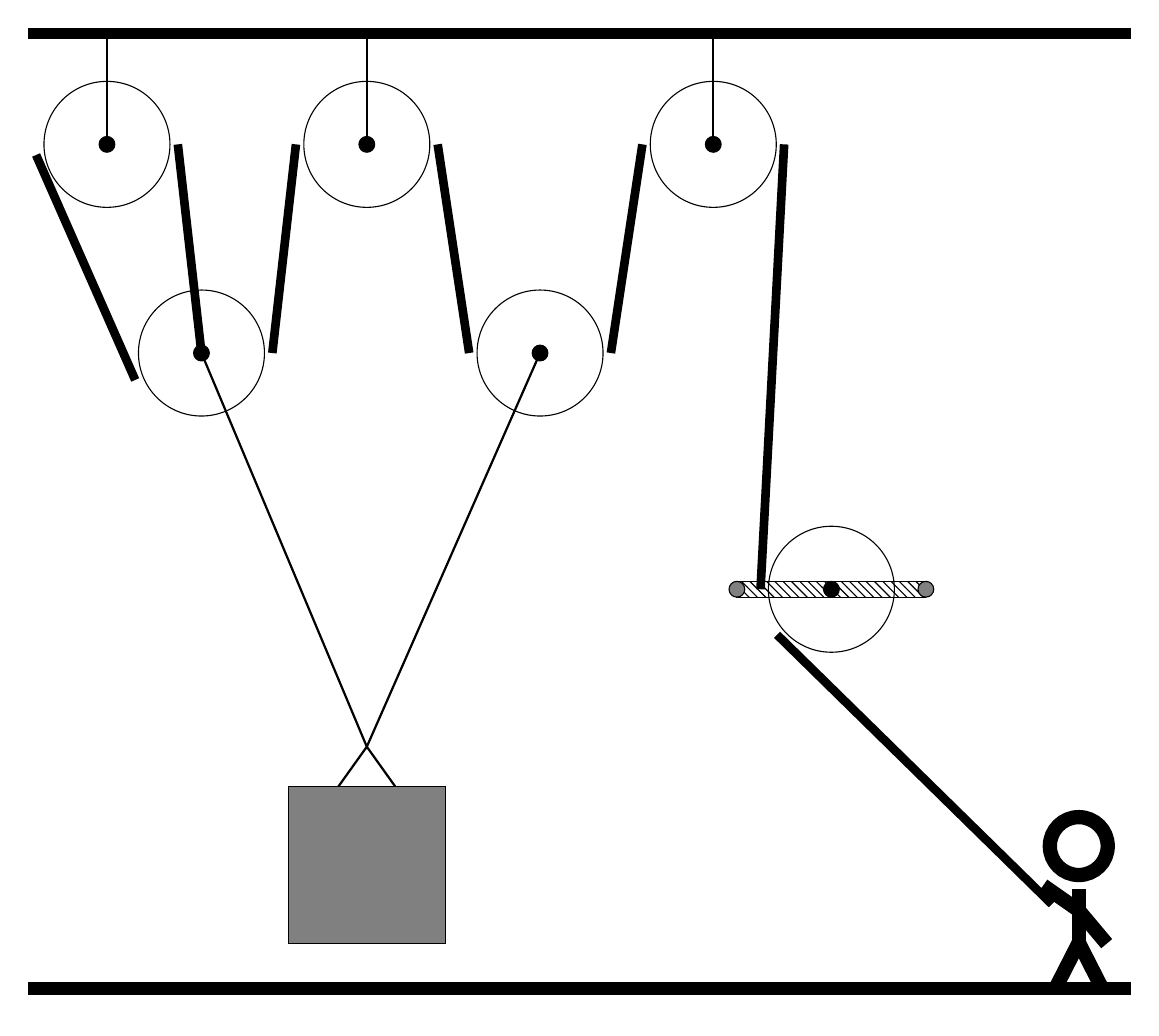
\begin{tikzpicture}
			%%%%% START %%%%%
			\draw[fill=black] (-2, 9) rectangle (12, 9.125);
			
			\draw (-1, 7.65) circle (0.8);
			\draw[fill=black] (-1, 7.65) circle (0.1);
			\draw[thick] (-1, 7.65) -- (-1, 9);
			
			\draw (2.3, 7.65) circle (0.8);
			\draw[fill=black] (2.3, 7.65) circle (0.1);
			\draw[thick] (2.3, 7.65) -- (2.3, 9);
			
			\draw (6.7, 7.65) circle (0.8);
			\draw[fill=black] (6.7, 7.65) circle (0.1);
			\draw[thick] (6.7, 7.65) -- (6.7, 9);
			
			\draw (0.2, 5) circle (0.8);
			\draw[fill=black] (0.2, 5) circle (0.1);
			
			\draw (4.5, 5) circle (0.8);
			\draw[fill=black] (4.5, 5) circle (0.1);
			
			\draw (8.2, 2) circle (0.8);
			\draw[fill=black] (8.2, 2) circle (0.1);
			\draw[pattern=north west lines, pattern color=black] (7.0, 2.1) rectangle (9.4, 1.9);
			\draw[fill=black!50] (7.0, 2) circle (0.1);
			\draw[fill=black!50] (9.4, 2) circle (0.1);
			
			\draw[thick] (0.2, 5) -- (2.3, 0)  -- (4.5, 5);
			\draw[thick]  (1.8, -0.7) -- (2.3, 0) -- (2.8, -0.7);
			\draw[fill=black!50] (1.3, -0.5) rectangle (3.3, -2.5);
			
			\draw[line width=1.1mm] (0.2, 5) -- (-0.1, 7.65);
			\centerarc[line width=1.1mm](-1, 7.65)(0:200:0.9);
			\draw[line width=1.1mm] (-1.9, 7.515) -- (-0.6415, 4.658);
			\centerarc[line width=1.1mm](0.2, 5)(200:360:0.9);
			\draw[line width=1.1mm](1.1, 5) -- (1.4, 7.65);
			\centerarc[line width=1.1mm](2.3, 7.65)(0:180:0.9);
			\draw[line width=1.1mm] (3.2, 7.65) -- (3.6, 5);
			\centerarc[line width=1.1mm](4.5, 5)(180:360:0.9);
			\draw[line width=1.1mm] (5.4, 5) -- (5.8, 7.65);
			\centerarc[line width=1.1mm](6.7, 7.65)(0:180:0.9);
			\draw[line width=1.1mm](7.6, 7.65) --  (7.3, 2);
			\centerarc[line width=1.1mm](8.2, 2)(180:220:0.9);
			\draw[line width=1.1mm](7.5106, 1.4215) -- (11, -2);
			
			\node at (11.3, -2) {\Strichmaxerl[10][-35][-50]};
			
			\draw[fill=black] (-2, -3) rectangle (12, -3.15);
			%%%%% END %%%%%
		\end{tikzpicture}
	\end{figure}	
\end{document}